\section{Methodik}

In diesem Abschnitt widmen wir uns den angewandten Methoden unserer Arbeit und erläutern die verwendeten Modelle sowie ihre Metriken und Algorithmen.

\subsection{Preprocessing}

Alle Bilder werden vor dem Training sowie nach dem Training und Evaluierung, wie folgt vorbereitet. \\

\begin{mdframed}
\begin{lstlisting}[language=python, label={ImagePreprocessor}, caption={Image Preprocessing}]

transform = torchvision.transforms.Compose(
    [
        torchvision.transforms.Resize((224, 224), antialias=True),
    ]
)

\end{lstlisting}
\label{code:preprocessing der Bilder}
\end{mdframed}

Die Bilder werden dabei auf eine Grösse von 224 Pixelhöhe und 224 Pixelbreite mit Antialiasing. 

Antialiasing ist eine Technik, die in der Computergrafik verwendet wird, um den Aliasing-Effekt zu entfernen. Der Aliasing-Effekt ist das Auftreten von gezackten Kanten oder "Jaggies" in einem gerasterten Bild.

\subsection{Modell Training}

\todo{Gabo}


\newpage
\subsection{UAP Algorithmus}

Unser Algorithmus für universelle adversarielle Perturbationen (UAP) basiert auf dem Ansatz von Moosavi-Dezfooli et al. \cite{moosavi-dezfooli_universal_2017}. Ziel ist es, eine Perturbation zu entwickeln, die auf neue Bilder übertragbar ist. Dies erreichen wir, indem wir iterativ durch eine Auswahl von Trainingsbildern gehen und den jeweils kürzesten Weg zur Entscheidungsgrenze jedes Bildes finden. Die dabei erzeugten Perturbationen werden summiert, um eine universelle Perturbation zu formen. 

\subsubsection{Loss-Funktion}
Das Optimierungsproblem wird bei unserer Umsetzung durch eine Loss-Funktion gelöst, welche die Norm der Perturbationsmatrix und die invertierte Binary Cross Entropy Funktion minimiert. Diese sieht wie folgt aus:

\begin{equation}
    L = \lambda_{norm} \cdot ||v + \Delta v||_p + \frac{1}{\text{BCE}(\hat{y}, \hat{y}_{adv}) + \epsilon}
\label{Loss}
\end{equation}

\begin{align*}
\text{Wobei:}&\\
L, &\text{ ist der gesamte Loss.} \\
\lambda_{norm}, &\text{ ist der Regularisierungsparameter.} \\
v, &\text{ ist die universelle Störung.} \\
\Delta v, &\text{ ist die Änderung der Störung.} \\
||v + \Delta v||_p, &\text{ repräsentiert die } L_p \text{-Norm der Perturbation } v + \Delta v. \\
\text{BCE}, &\text{ bezeichnet den Binary-Cross-Entropy Loss.} \\
\hat{y}, &\text{ ist die Vorhersage des Modells für das Originalbild.} \\
\hat{y}_{adv}, &\text{ ist die Vorhersage des Modells für das perturbierte Bild.} \\
\epsilon, &\text{ ist eine kleine positive Konstante für numerische Stabilität.}
\end{align*}


Für $\epsilon$ wird ein kleiner Wert wie $1^{-6}$ gewählt, der eine Division durch Null verhindert, wenn der Output unseres Modells sowohl mit als auch ohne Störung gleich ist. Dies ist vorallem bei der Berechnung der allerersten Perturbation ein Problem.

\newpage
\subsubsection{Technische Umsetzung}
Die technische Umsetzung des Prozesses zur Generierung der UAP-Bilder ist in der folgenden Grafik \ref{fig:05-uap_algorithm} dargestellt:

\begin{figure}[H]
    \centering
    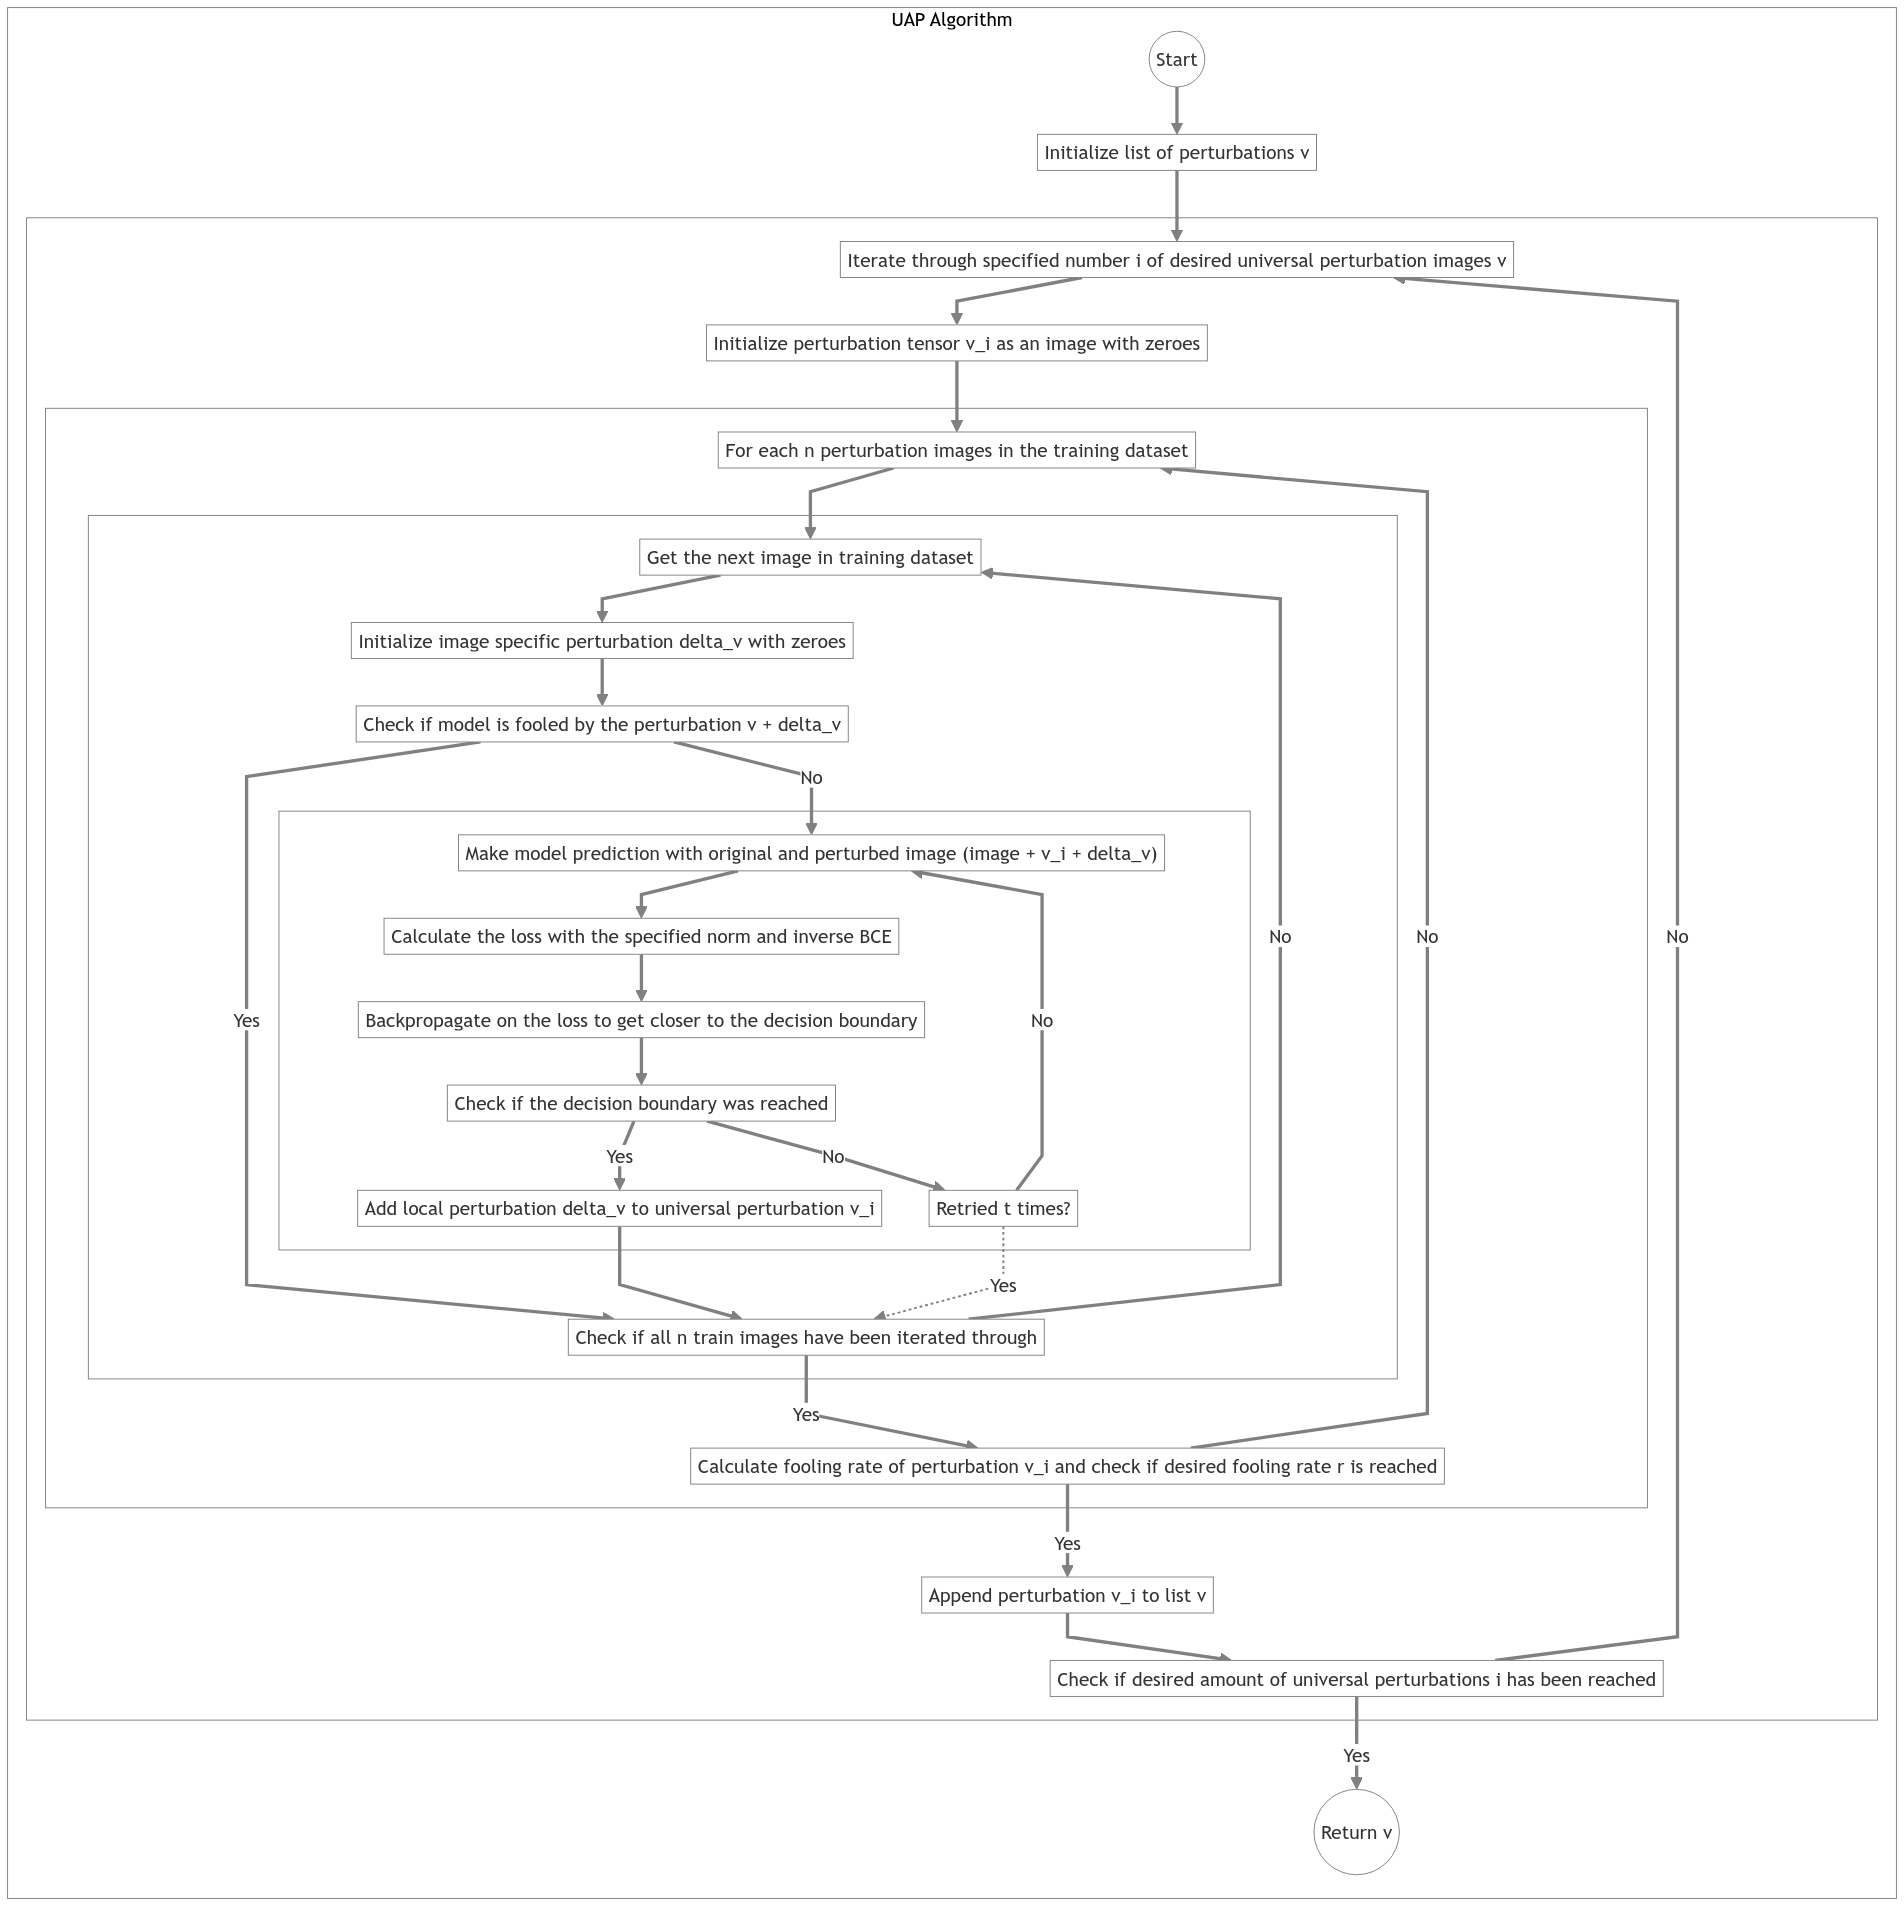
\includegraphics[width=14.5cm]{01-images/05-UAP_ALG}
    \caption{UAP Algorithmus}
    \label{fig:05-uap_algorithm}
\end{figure}


\text{Wobei man folgende Parameter selbst bestimmen muss:}
\begin{align*}
i, &\text{ ist die Anzahl Perturbationsbilder, welche generiert werden sollen.} \\
n, &\text{ ist die Anzahl Trainingsbilder, welche für die Generierung verwendet werden.} \\
t, &\text{ ist die Anzahl Versuche, eine bildlokale Perturbation zu finden}\\
r, &\text{ ist der prozentuelle Anteil von Trainingsbilder, welche durch die Perturbationen} \\ 
&\text{  getäuscht werden soll, damit die Perturbation } v_i \text{ gespeichert wird.} \\
p, &\text{ ist der Normparameter der } L_p \text{ Norm.}\\
\lambda_{norm}, &\text{ siehe Loss-Funktion.}\\
\epsilon, &\text{ siehe Loss-Funktion.}
\end{align*}